\section*{VDM's}
\begin{frame}{Variational Diffusion Models (VDM's)}
    Variational Diffusion Model (VDM) is simply a MHVAE with 3 restrictions:
    \begin{enumerate}
        \item The dimension of latent variables is equal to dimension of data.
        \item Distribution of latent variables at each time step is Gaussian Centered at latent variable at previous time step. (This is not learnt, but fixed)
        \item Encoding transitions are done in such a way that distribution of latent variable at last time step is standard Gaussian.
    \end{enumerate}

    Let us see what changes occur in MHVAE when these restrictions are applied to it.
\end{frame}

\begin{frame}{Variational Diffuion Models (VDM's)}
    \begin{figure}
        \centering
        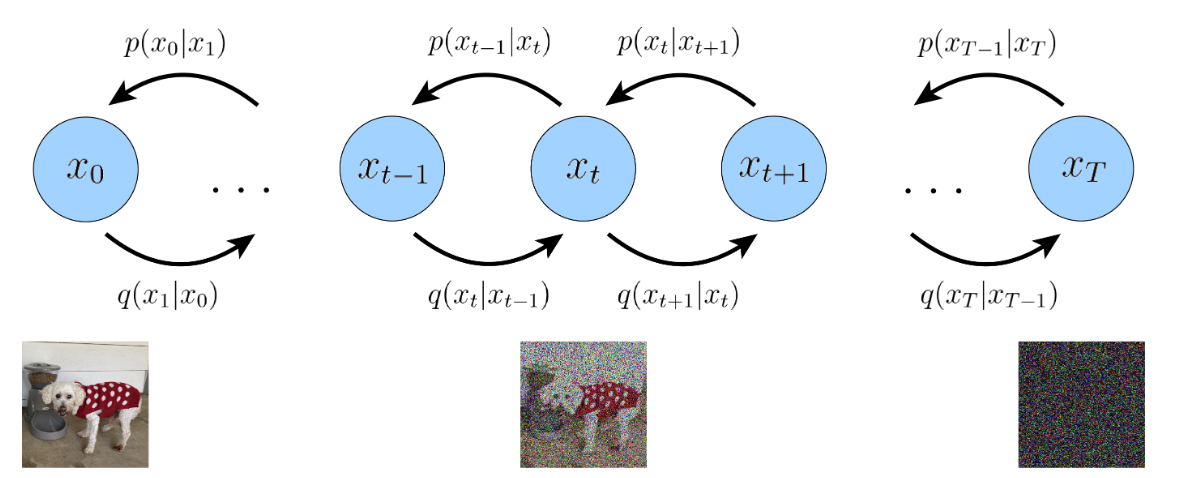
\includegraphics[width=1\textwidth]{Images/vdm1.png}
        \caption{Variational Diffusion Model}
    \end{figure}
\end{frame}

\begin{frame}{Variational Diffusion Models (VDM's)}
    \begin{itemize}
        \item $x_0$ represents true data observations.
        \item $x_t$ represents intermediate noisy version of data.
        \item $x_T$ represents pure Gaussian noise.
    \end{itemize}
\end{frame}

\begin{frame}{Restriction 1}
    According to slight change of notation in previous slide, VDM's posterior is same as MHVAE's posterior which can now be written as:
    \begin{align*}
        q(x_{1:T}|x_0) &= \prod_{t=1}^{T} q(x_t|x_{t-1}) && \text{(VDM's Posterior)}
    \end{align*}
    instead of 
    \begin{align*}
        q(z_{1:T}|x) &= p(z_1|x) \prod_{t=2}^{T} q(z_t|z_{t-1}) && \text{(MHVAE's Posterior)}
    \end{align*}
\end{frame}

\begin{frame}{Restriction 2}
    Unlike MHVAE, distribution of latent variable at each time step is not learnt, but is fixed. Mathematically, the encoder transitions can be written as:
    \begin{align*}
        q(x_t|x_{t-1}) &= \mathcal{N}(x_t; \sqrt{\alpha_t}x_{t-1}, (1-\alpha_t) \mathbb{I}_{d \times d}) 
    \end{align*}

    Distribution of latent variable $x_t$ at each time step is gaussian centered at latent variable at previous time step $x_{t-1}$.
\end{frame}

\begin{frame}{Restriction 3}
    Gaussian Transitions are made in such a way that distribution of final latent variable $x_T$ is standard Gaussian. Mathematically, this can be written as:
    \begin{align*}
        q(x_T|x_{T-1}) &= \mathcal{N}(x_T; 0, \mathbb{I}_{d \times d})
    \end{align*}

    Hence Joint Distribution of VDM can be written as:
    \begin{align*}
        p(x_{0:T}) &= p(x_T) \prod_{t=1}^{T} q(x_{t-1}|x_{t}) && p(x_T) \sim \mathcal{N}(0, \mathbb{I}_{d \times d})
    \end{align*}
    Instead of
    \begin{align*}
        p(x,z_{1:T}) &= p(x_T)p(x|z_1) \prod_{t=2}^{T} q(z_{t-1}|z_{t}) && \text{(MHVAE's Joint)}
    \end{align*}
\end{frame}

\begin{frame}{Learning conditionals}
    Since encoder transitions are fixed for each time steps, we are only interested in learning conditionals $p(x_{t-1}|x_t)$ so that we can simulate new data. 

    \bigskip

    We can achieve this by maximizing ELBO for VDM. To show that maximizing ELBO actually helps in learning conditionals, we will first split ELBO in different components like we did in VAE and got the reconstruction term and prior matching term.
\end{frame}

\begin{frame}{Breaking down ELBO}
    We know that ELBO for MHVAE can be written as:
    \begin{align*}
        ELBO &=  \mathbb{E}_{q(z_{1:T}|x)} \left[ \log \left( \frac{p(x, z_{1:T})}{q(z_{1:T}|x)} \right) \right] \\
    \end{align*}
    According to notation's for VDM, we can write ELBO as:
    \begin{align*}
        ELBO &=  \mathbb{E}_{q(x_{1:T}|x_0)} \left[ \log \left( \frac{p(x_{0:T})}{q(x_{1:T}|x_0)} \right) \right] \\
    \end{align*}
\end{frame}

\begin{frame}{Breaking down ELBO}
    We further saw that ELBO for MHVAE can be written as:
    \begin{align*}
        ELBO &= &= \mathbb{E}_{q(z_{1:T}|x)} \left[ \log \left( \frac{p(z_T)p(x|z_1) \prod_{t=2}^{T} p(z_{t-1}|z_t)}{q(z_1|x) \prod_{t=2}^{T} q(z_t|z_{t+1})} \right) \right] \\
    \end{align*}

    In our case we can write this as:
    \begin{align*}
        ELBO &= \mathbb{E}_{q(x_{1:T}|x_0)} \left[ \log \left( \frac{p(x_T) \prod_{t=1}^{T} p(x_{t-1}|x_t)}{\prod_{t=1}^{T} q(x_t|x_{t-1})} \right) \right] \\
    \end{align*}

    Let us now further simplify this expression.
\end{frame}

\begin{frame}{Breaking down ELBO}
    \begin{align*}
        ELBO &= \mathbb{E}_{q(x_{1:T}|x_0)} \left[ \log \left( \frac{p(x_T) \prod_{t=1}^{T} p(x_{t-1}|x_t)}{\prod_{t=1}^{T} q(x_t|x_{t-1})} \right) \right] \\
        &= \mathbb{E}_{q(x_{1:T}|x_0)} \left[ \log \left( \frac{p(x_T)p(x_0|x_1) \prod_{t=2}^{T} p(x_{t-1}|x_t)}{\prod_{t=1}^{T} q(x_t|x_{t-1})} \right) \right] \\
        &= \mathbb{E}_{q(x_{1:T}|x_0)} \left[ \log \left( \frac{p(x_T)p(x_0|x_1) \prod_{t=2}^{T} p(x_{t-1}|x_t)}{q(x_T|x_{T-1}) \prod_{t=1}^{T-1} q(x_t|x_{t-1})} \right) \right] \\
        &= \mathbb{E}_{q(x_{1:T}|x_0)} \left[ \log \left( \frac{p(x_T)p(x_0|x_1) \prod_{t=1}^{T-1} p(x_{t}|x_{t+1})}{q(x_T|x_{T-1}) \prod_{t=1}^{T-1} q(x_t|x_{t-1})} \right) \right] \\
    \end{align*}
\end{frame}

\begin{frame}{Breaking down ELBO}
    \begin{align*}
        &= \mathbb{E}_{q(x_{1:T}|x_0)} \left[ \log \left( \frac{p(x_T)p(x_0|x_1)}{q(x_T|x_{T-1})} \right) + \sum_{t=1}^{T-1} \log \left( \frac{p(x_{t}|x_{t+1})}{q(x_t|x_{t-1})} \right) \right] \\
        &= \mathbb{E}_{q(x_{1:T}|x_0)} \left[ \log \left( \frac{p(x_T)p(x_0|x_1)}{q(x_T|x_{T-1})} \right) \right] + \sum_{t=1}^{T-1} \mathbb{E}_{q(x_{1:T}|x_0)} \left[ \log \left( \frac{p(x_{t}|x_{t+1})}{q(x_t|x_{t-1})} \right) \right] \\
    \end{align*}

    First Term can further be simplified into
    \begin{align*}
        &= \mathbb{E}_{q(x_{1:T}|x_0)} \left[ \log \left( \frac{p(x_T)}{q(x_T|x_{T-1})} \right) \right] + \mathbb{E}_{q(x_{1:T}|x_0)} \left[ \log \left( p(x_0|x_1) \right) \right] \\
    \end{align*}
\end{frame}